\setcounter{page}{1}
\pagenumbering{arabic}
\chapter{Inleiding}
\label{ch:Inleiding}
Menselijke actieherkenning is het proces dat op een automatische manier (I) detecteert dat een persoon een bepaalde actie uitvoert en (II) herkennen welke actie dit is. Voorbeelden van zulke acties zijn lopen, stappen, zwaaien, springen, bukken, enz. Actieherkenning kent tal van toepassingen, voornamelijk bij de interactie tussen mens en computer, zoals fysiotherapie \cite{Deboeverie2016}, lichaamsanalyse \cite{Devi2015} en \todo{nog wat voorbeelden zoeken}

Actieherkenning wordt voornamelijk gerealiseerd met kleuren- en dieptebeelden.







\section{Probleemstelling}
In het onderzoeksgebied actieherkenning is er al uitbundig onderzoek gedaan. Zo is men in staat om voor zowel kleurenbeelden als dieptebeelden actieherkenning toe te passen op een betrouwbare manier. Echter blijft het moeilijk om dit te realiseren in een real-time scenario, waarbij snelle beslissingen gemaakt moeten worden. Een groot probleem is de onzekerheid van de actie. In de literatuur worden er vaak methoden (\cite{Xia2012}, ...) beschreven die acties herkennen op video's waarop slechts één actie uitgevoerd wordt. De actielabel wordt ook maar nadien toegekend, als de video gedaan is. Een betere aanpak zou de actielabel toekennen op het moment dat de actie bezig is, op een video waarbij meerdere acties kunnen uitgevoerd worden op hetzelfde moment, of verschillende acties op andere momenten en met een achtergrond die irrelevant kan zijn. In de literatuur worden dit \textit{untrimmed video's} genoemd. In zulke video's zijn de actielabels, actiepositie en actieduur onbekende parameters.

 De THUMOS Challenge \footnote{\url{http://www.thumos.info}} werd georganiseerd in 2015 en was een initiatief om op een competitieve manier het probleem van actieherkenning in untrimmed video's te onderzoeken. Ze bieden een dataset aan met untrimmed video's die scenario's uit het echte leven bevatten. Het doel van deze masterproef is om eerst te onderzoeken welke methoden er al bestaan op vlak van actieherkenning in untrimmed video's en hoe deze aangepast kunnen worden zodat ze werken op de skeletdata van een Kinect. De complete oplossingsstrategie wordt beschreven in hoofdstuk \ref{ch:methodologie}.



\section{De Kinect}
De Kinect (figuur \ref{fig:KinectSensorVersies}) is origineel ontworpen als manier om de gebruiker zelf als spelcontroller te beschouwen. Dit is een grote vordering in vergelijking met de Eyetoy, die geen dieptezicht heeft of de Wii Remote, waarbij de gebruiker een controller moet hebben om acties uit te voeren. Door de combinatie van de diepte- en kleurenbeelden die de Kinect kan leveren kunnen er skeletbeelden gegenereerd worden. Voor elke frame kan de Kinect tot maximaal 25 skeletjoints genereren, voor maximaal zes personen, die drie-dimensionale coördinaten voorstellen van voornamelijk gewrichten van het lichaam. Dit speelt een groot voordeel: het detecteren van de low-level features om de skeletjoints te bepalen wordt overgelaten aan de Kinect zelf. Sindsdien is het onderzoek naar actieherkenning met behulp van skeletjoints terug in leven geschoten.

Ondanks het succes van de Kinect heeft Microsoft toch besloten om het product niet meer als entertainmentproduct te verkopen, maar wel als een tool die onderzoekers en ontwikkelaars kunnen helpen. De volgende versie van de Kinect draagt de naam Azure Kinect en is rechtstreeks verbonden met het Azure platform van Microsoft. In deze masterproef wordt de tweede versie van de Kinect gebruikt (figuur \ref{fig:KinectSensorOne}).

\begin{figure}
	\begin{subfigure}[t]{0.48\textwidth}
		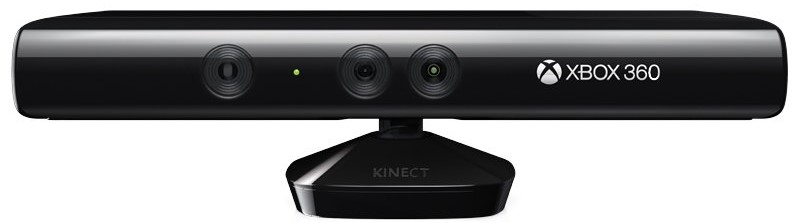
\includegraphics[width=\linewidth]{KinectSensor360}
		\caption{De originele Kinect sensor, ontwikkeld int 2010 voor de Xbox 360.}
	\end{subfigure}
	\begin{subfigure}[t]{0.48\textwidth}
		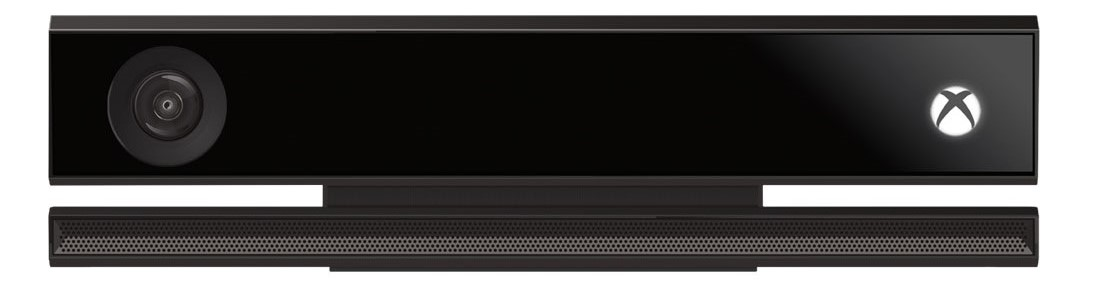
\includegraphics[width=\linewidth]{KinectSensorOne}
		\caption{De tweede iteratie van de Kinect sensor, specifiek gemaakt voor Xbox One en uitgebracht in 2013.}
		\label{fig:KinectSensorOne}
	\end{subfigure}
	\caption{Twee versies van de Kinect sensor.}
	\label{fig:KinectSensorVersies}
\end{figure}




\section{Structuur}
In hoofdstuk \ref{ch:methodologie} wordt de algemene methodologie beschreven die gebruikt wordt om deze masterproef te realiseren, waarom deze gebruikt wordt en wat het beoogde eindresultaat is. Verder wordt er in hoofdstuk \ref{ch:literatuur} een overzicht gegeven van bestaande methoden en welke features en classifiers zij gebruiken.
